\thispagestyle{timhieukhoahocnone}
\pagestyle{timhieukhoahoc}
\everymath{\color{timhieukhoahoc}}
\blfootnote{$^1$\text{\color{timhieukhoahoc}Hà Nội.}}
\graphicspath{{../timhieukhoahoc/pic/}}
\begingroup
\AddToShipoutPicture*{\put(0,616){\includegraphics[width=19.3cm]{../bannertimhieu}}}
\AddToShipoutPicture*{\put(86,520){\includegraphics[scale=1]{../tieude.pdf}}}
\centering
\endgroup
\vspace*{185pt}

\begin{multicols}{2}
	Pascal không chỉ là một nhà toán học lớn mà còn có nhiều đóng góp trong ngành vật lý. Nhân dịp kỷ niệm $400$ năm ngày sinh của Pascal ($1623-2023$), chúng ta hãy cùng Pi tìm hiểu nguyên lý mang tên ông về áp suất trong lòng chất lỏng cùng những thí nghiệm của Pascal xung quanh vấn đề này.
	\begin{figure}[H]
		\vspace*{-5pt}
		\centering
		\captionsetup{labelformat= empty, justification=centering}
		\includegraphics[width= 0.7\linewidth]{1}
		\caption{\small\textit{\color{timhieukhoahoc}Blaise Pascal $(1623-1662)$.}}
		\vspace*{-10pt}
	\end{figure}
	$\pmb{1.}$ \textbf{\color{timhieukhoahoc}Các thí nghiệm của Pascal về áp suất trong chất lỏng}
	\vskip 0.1cm
	Từ năm $1644$, khi Torricelli tiến hành đo áp suất khí quyển với áp kế thủy ngân, nhiều nhà khoa học khác ở châu Âu cũng bắt đầu quan tâm đến vấn đề này. Các tranh cãi chủ yếu xoay quanh sự tồn tại của chân không cũng như sự thay đổi của áp suất theo độ cao. Nhiều thí nghiệm được thực hiện ở Pháp bởi Pascal cũng như Roberval để kiểm chứng các nhận định đã có cũng như đưa ra các kết quả mới. Bạn đọc có thể xem lại các vấn đề về áp suất khí quyển liên quan đến Pascal và Torricelli trong Pi số $11$ năm $2020$.
	\begin{figure}[H]
		\vspace*{-5pt}
		\centering
		\captionsetup{labelformat= empty, justification=centering}
		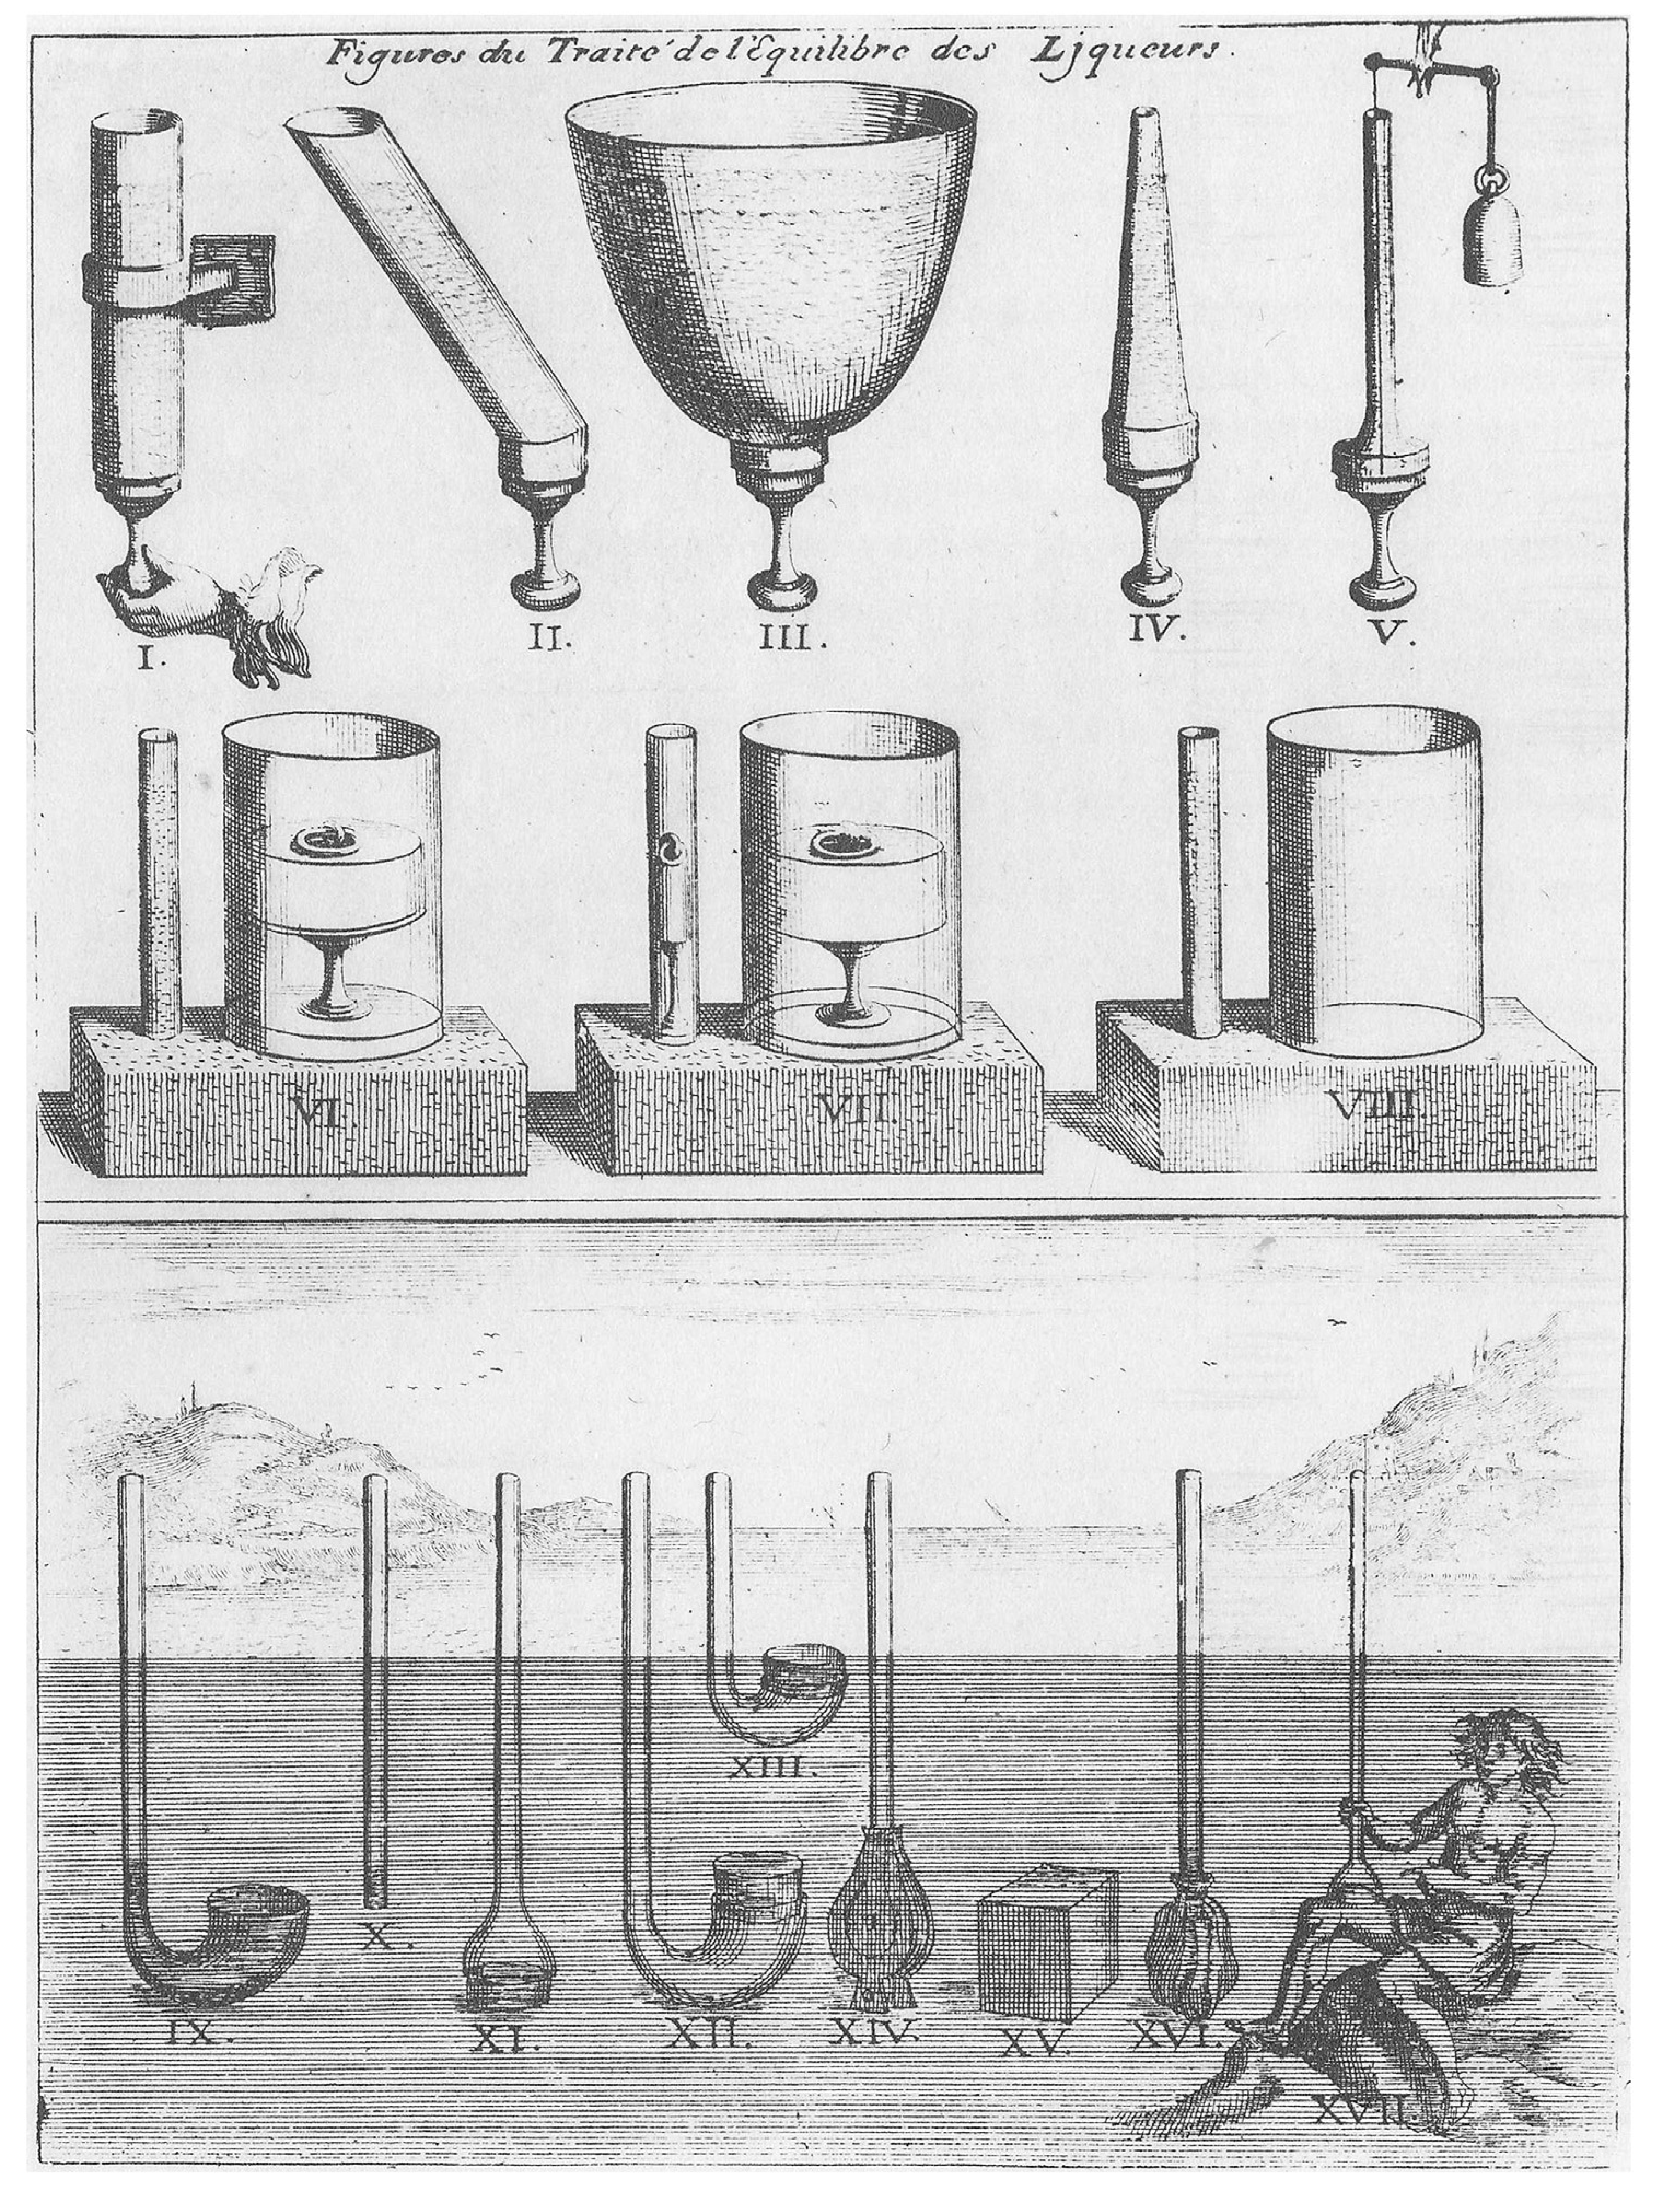
\includegraphics[width= 1\linewidth]{2}
		\caption{\small\textit{\color{timhieukhoahoc}Hình $1$. Bảng hình vẽ số $1$ trong Traité de l'équilibre des liqueurs của Pascal.}}
		\vspace*{-5pt}
	\end{figure}
	Không chỉ dừng lại ở áp suất khí quyển, Pascal còn tiếp tục nghiên cứu sâu hơn về áp suất ở trong lòng của một chất lỏng. Cuốn sách \textit{Traité de l'équilibre des liqueurs (Về sự cân bằng của chất lỏng)} của ông đã trình bày nhiều thí nghiệm đa dạng về chủ đề này. Những thí nghiệm liên quan được ông tổng kết trong một hình vẽ tóm tắt (Hình $1$).
	\begin{figure}[H]
		\vspace*{-5pt}
		\centering
		\captionsetup{labelformat= empty, justification=centering}
		\includegraphics[width= 0.95\linewidth]{3}
		\caption{\small\textit{\color{timhieukhoahoc}Hình $2$. Với cùng một mực chất lỏng, áp suất ở đáy bình với các hình dạng khác nhau đều sẽ bằng nhau.}}
		\vspace*{-10pt}
	\end{figure}
	Các thí nghiệm I đến IV minh họa phát biểu thứ nhất của Pascal về áp suất trong lòng chất lỏng: áp suất do chất lỏng gây ra phụ thuộc vào độ cao của cột chất lỏng và độc lập với tổng khối lượng của chất lỏng. Các bình chứa với hình dạng khác nhau được đổ nước đến cùng một độ cao và khi đó áp suất tại vị trí được bịt lại ở đáy của chúng đều bằng nhau (Hình $2$). Thí nghiệm V mô tả cách đo áp suất này.
	\begin{figure}[H]
		\vspace*{-10pt}
		\centering
		\captionsetup{labelformat= empty, justification=centering}
		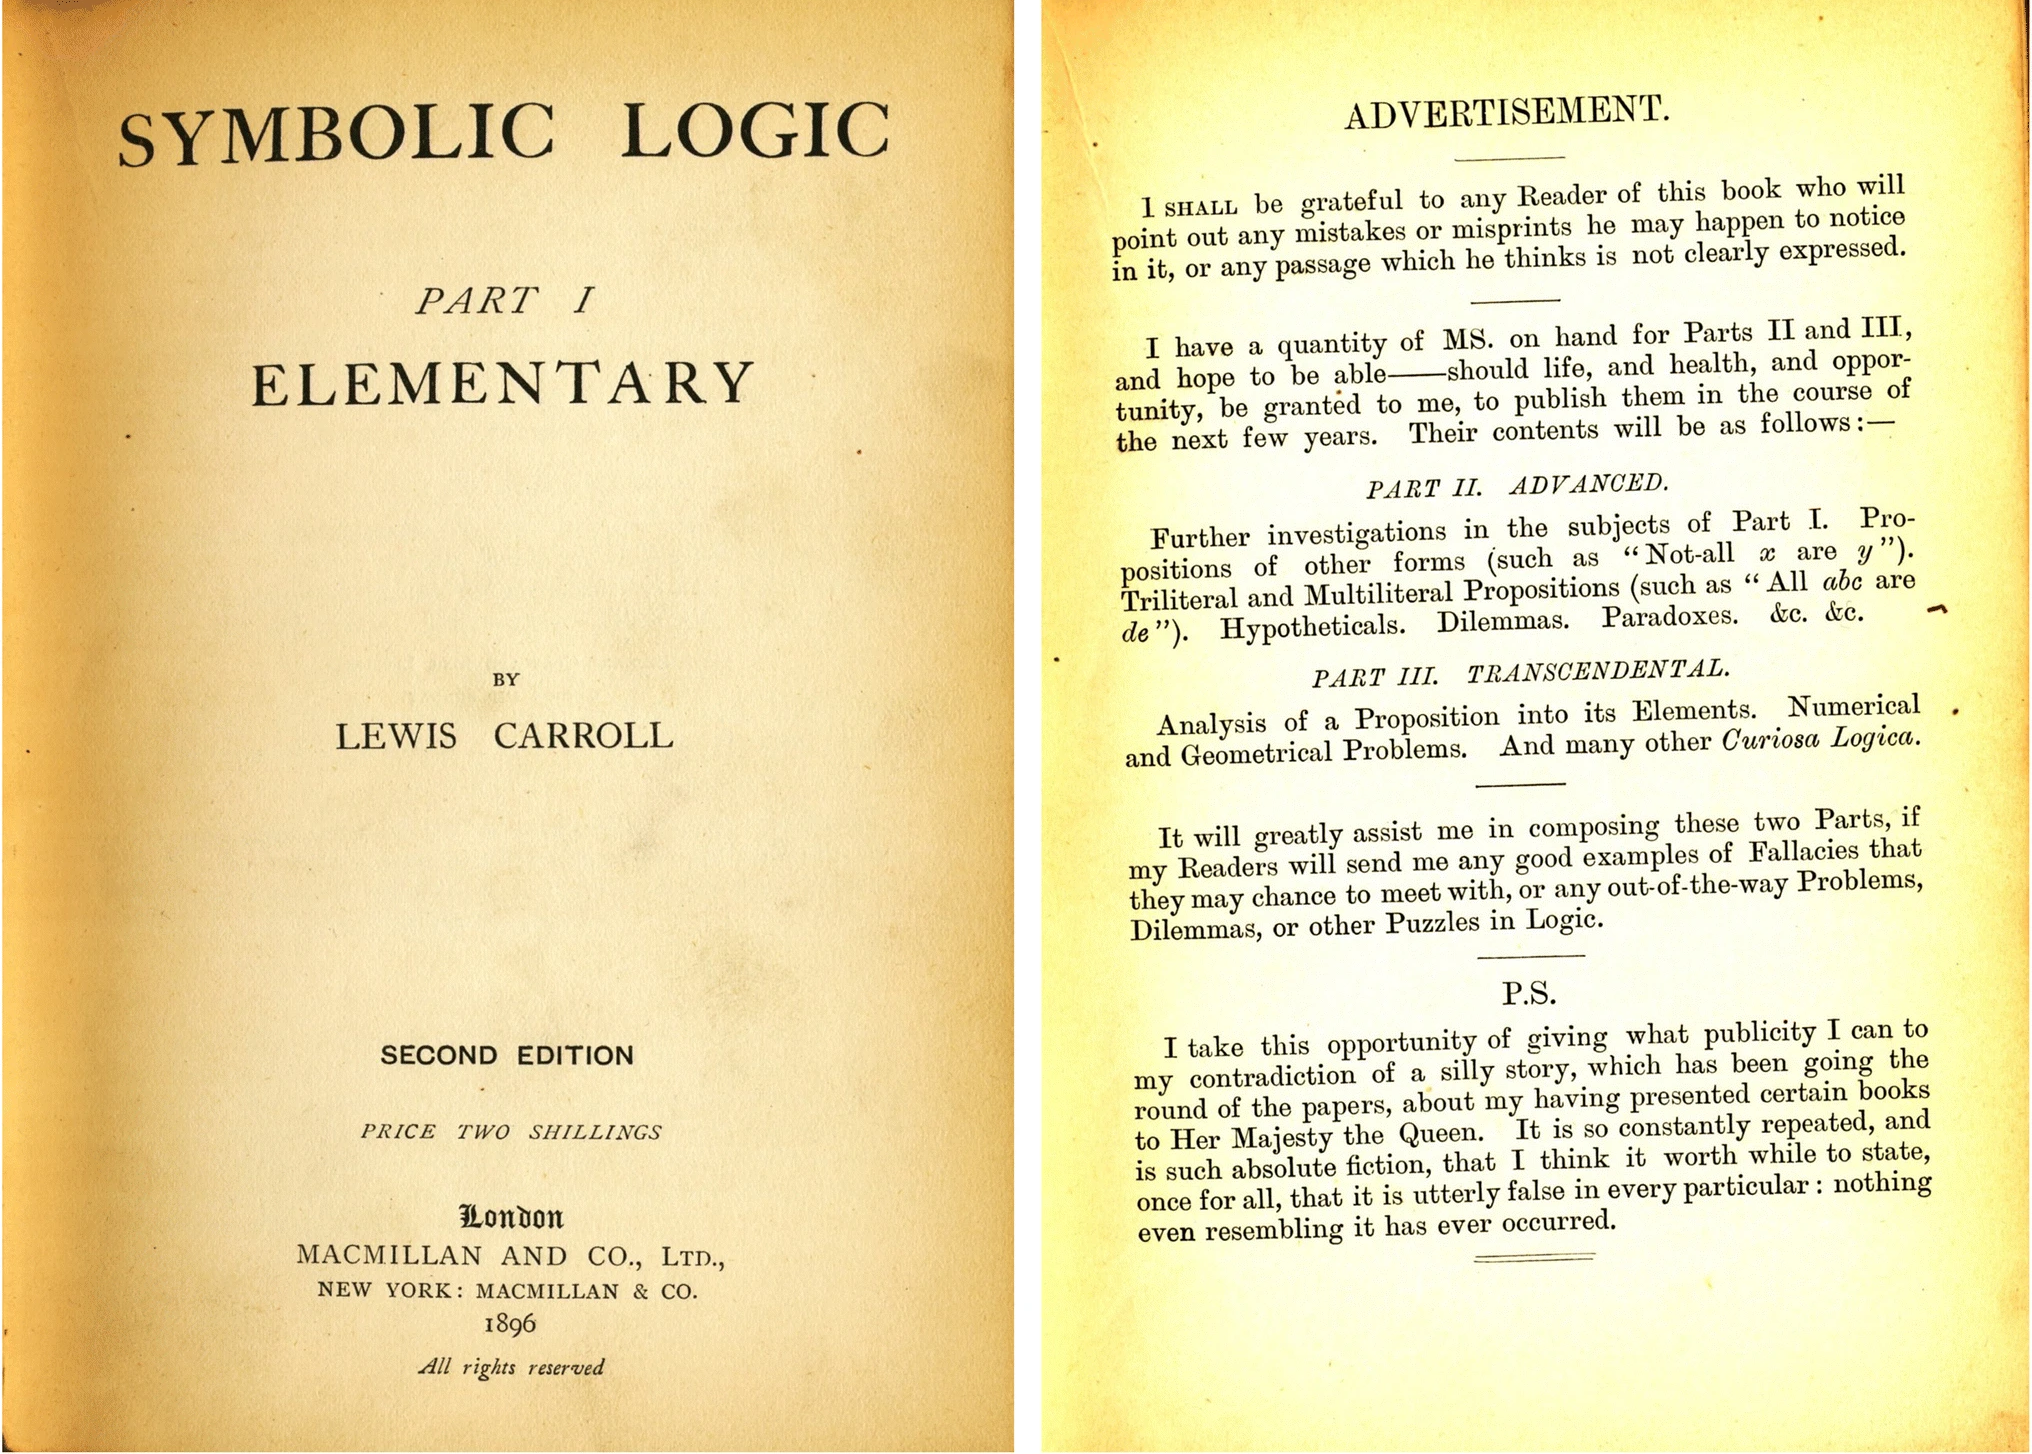
\includegraphics[width= 0.85\linewidth]{4}
		\caption{\small\textit{\color{timhieukhoahoc}Hình $3$. Sơ đồ thí nghiệm đo áp suất ở đáy bình tương tự như trong thí nghiệm V. Lực do áp suất nước tác dụng lên khối chặn ở đáy bình sẽ cân bằng với trọng lượng của các vật trên đĩa cân ở phía đối diện.}}
		\vspace*{-5pt}
	\end{figure}
	Trong thí nghiệm V, bình chứa có dạng một ống hẹp với lỗ mở to ở đáy. Một khối chặn ở đáy bình được nối với một đòn bẩy có một quả cân ở phía đối diện sao cho hai tay đòn bằng nhau. Khi lực do áp suất nước tác dụng lên khối chặn và trọng lực của quả cân cân bằng với nhau ở hai phía của đòn bẩy, ta có thể thiết lập được sự phụ thuộc giữa áp suất và độ cao của cột nước. Nếu với cũng lượng nước đó nhưng được làm cho đông đặc thì khối lượng của quả cân chỉ bằng $1/100$ so với trường hợp nước lỏng. Do đó, quan hệ về áp suất và chiều cao ở trên chỉ áp dụng với chất lỏng và không đúng với chất rắn.
	\begin{figure}[H]
		\vspace*{-5pt}
		\centering
		\captionsetup{labelformat= empty, justification=centering}
		\includegraphics[width= 0.8\linewidth]{5}
		\caption{\small\textit{\color{timhieukhoahoc}Hình $4$. Thí nghiệm VI của Pascal: một cột nước ở một nhánh của bình chứa cân bằng với một pít tông ở nhánh còn lại.}}
		\vspace*{-10pt}
	\end{figure}
	Trong thí nghiệm VI, Pascal sử dụng một bình chứa có hai lỗ ở mặt trên, lỗ bé có diện tích chỉ bằng $1/100$ diện tích của lỗ lớn. Ở mỗi lỗ, ta gắn một ống kim loại. Nếu ống nhỏ được đổ đầy nước và một pít tông được đặt trên ống còn lại thì pít tông cần có khối lượng rất lớn để ngăn cho nước không đẩy lên. Cách đo này tương tự như việc sử dụng quả cân để đo áp suất ở đáy bình chứa trong thí nghiệm V. Điều khác biệt là lúc này áp suất tạo lực đẩy hướng lên trên. Nếu cột nước bên ống nhỏ có chiều cao tăng gấp đôi thì khối lượng của pít tông cần đặt bên ống lớn cũng phải tăng gấp đôi. Những kết quả quan sát vẫn đúng ngay cả khi pít tông chặn được đặt ở mặt bên của bình chứa. Pascal tổng kết các thí nghiệm trên bằng kết luận: \textit{áp suất do cột nước gây ra phụ thuộc vào độ cao của nó}, chứ không phải độ rộng.
	\vskip 0.1cm
	\PIbox{Công thức cho sự phụ thuộc của áp suất theo độ sâu là: $p=\rho gh$ với $\rho$ là khối lượng riêng của chất lỏng còn $g$ là gia tốc trọng trường$^2$.}
	\vskip 0.1cm
	Trong thí nghiệm VII, cột nước ở ống bé cũng được thay bằng một pít tông để cân bằng với pít tông bên ống lớn. Tỷ lệ khối lượng $2$ pít tông cũng bằng tỷ lệ của diện tích hai lỗ, tức là pít tông ở lỗ nhỏ chỉ cần có khối lượng bằng $1/100$ pít tông ở lỗ lớn. Nếu ta ấn một pít tông thì cái còn lại sẽ dịch chuyển một đoạn tương ứng ngược với tỷ lệ diện tích: nếu ta dịch chuyển pít tông ở lỗ nhỏ một đoạn thì pít tông ở lỗ lớn chỉ dịch đi một đoạn bằng $1/100$ đoạn này mà thôi. Như Pascal đã giải thích, tính không nén được của nước làm cho thể tích nước bị dịch chuyển ở hai phía là như nhau. Pascal đã liên hệ sự tương quan này với các máy cơ học đơn giản khác như đòn bẩy và ròng rọc, trong đó nếu ta lợi về lực thì sẽ phải chịu đoạn dịch chuyển dài hơn và ngược lại. Nói cách khác thì tích của lực và đường đi luôn không đổi, hay công sẽ không đổi.
	\begin{figure}[H]
		\vspace*{-5pt}
		\centering
		\captionsetup{labelformat= empty, justification=centering}
		\includegraphics[width= 0.8\linewidth]{6}
		\caption{\small\textit{\color{timhieukhoahoc}Hình $5$. Thí nghiệm VII của Pascal: Sự cân bằng áp suất của hai pít tông. Hai pít tông có khối lượng khác nhau nhưng tỷ lệ với diện tích thiết diện ống sẽ cân bằng nhau ở hai nhánh của bình chứa.}}
		\vspace*{-10pt}
	\end{figure}
	\blfootnote{$^2$\color{timhieukhoahoc}Vào thời của Pascal, vật lý chưa có khái niệm về áp suất cũng như gia tốc trọng trường. Pascal đã đưa ra khái niệm lực trên một đơn vị diện tích nhưng chưa gọi nó là áp suất.}
	\!\!Khi so sánh thí nghiệm VI và VII, Pascal nhận thấy sự tương đương giữa cột nước ở VI và pít tông bên ống bé ở VII, chúng có cùng khối lượng. Phân tích tương tự cũng có thể áp dụng cho thí nghiệm V: cột nước ở phần ống có thiết diện bé tương đương với một pít tông sao cho khối lượng của nó và quả cân sẽ tỷ lệ với tỷ số diện tích của ống và diện tích phần đáy.
	\vskip 0.1cm
	Những thí nghiệm nảy giúp Pascal đưa ra một phát biểu quan trọng thứ hai: \textit{áp suất do cột nước hoặc một lực bên ngoài gây ra sẽ được truyền nguyên vẹn trong lòng chất lỏng theo mọi hướng}. Pascal giải thích rằng hiện tượng này xảy ra do tính liên tục và tính lỏng của các chất lỏng.
	\vskip 0.2cm
	\PIbox{
	\begin{figure}[H]
		\vspace*{-10pt}
		\centering
		\captionsetup{labelformat= empty, justification=centering}
		\includegraphics[width= 1\linewidth]{7}
		\vspace*{-20pt}
	\end{figure}
	Ngày nay ta đã biết hiện tượng trong phát biểu trên của Pascal có nguyên nhân là do cấu tạo ở cấp độ phân tử của chất lỏng. Trong khi chất rắn có các phân tử chỉ dịch chuyển được quanh các vị trí cố định thì các phân tử chất lỏng có thể dịch chuyển tự do hơn nhưng vẫn liên kết với nhau. Do đó, chất lỏng có thể thay đổi hình dạng nhưng thể tích không thay đổi. Việc này dẫn đến chất lỏng không nén được và áp suất sẽ được truyền đi trong lòng nó theo tương tác giữa các phân tử. Còn với chất khí, các phân tử chuyển động hỗn loạn không ngừng và hoàn toàn có thể tách rời nhau nên áp suất sẽ không được truyền đi nguyên vẹn mà phụ thuộc vào các định luật về chất khí như trong phần nhiệt học của sách giáo khoa Vật lý lớp $10$.}
	\vskip 0.2cm
	Cuốn sách của Pascal còn trình bày nhiều thí nghiệm khác nhau liên quan đến phát biểu trên. 
	\begin{figure}[H]
		\vspace*{5pt}
		\centering
		\captionsetup{labelformat= empty, justification=centering}
		\includegraphics[width= 0.75\linewidth]{8}
		\caption{\small\textit{\color{timhieukhoahoc}Hình $6$. Thí nghiệm VIII của Pascal: Hai cột chất lỏng ở hai nhánh của bình thông nhau luôn có mực chất lỏng bằng nhau khi cân bằng.}}
		\vspace*{-10pt}
	\end{figure}
	Trong thí nghiệm VIII, cả hai pít tông đều được thay bằng các ống thẳng chứa nước. Hệ cân bằng khi mực nước ở cả hai ống ngang bằng nhau. Quan hệ giữa khối lượng của chúng cũng giống như trong trường hợp hai pít tông: tỷ lệ với diện tích của lỗ ở mỗi ống. Đây cũng chính là \textit{bình thông nhau} mà ta đã quen thuộc trong sách giáo khoa vật lý. Nếu ta sử dụng hai chất lỏng khác nhau, ví dụ như nước và thủy ngân, ở mỗi bên ống, chúng sẽ cân bằng khi chiều cao của hai cột chất lỏng tỷ lệ nghịch với mật độ của chúng.
	\begin{figure}[H]
		\vspace*{-5pt}
		\centering
		\captionsetup{labelformat= empty, justification=centering}
		\includegraphics[width= 0.75\linewidth]{9}
		\caption{\small\textit{\color{timhieukhoahoc}Hình $7$. Với bình thông nhau có nhiều nhánh, mực chất lỏng ở các nhánh cũng vẫn luôn bằng nhau.}}
		\vspace*{-10pt}
	\end{figure}
	Tính đẳng hướng của việc lan truyền áp suất cũng được thể hiện ở việc khi cho một ống thẳng vào nước với đầu trên và đầu dưới đều hở, độ cao của cột thủy ngân trong ống độc lập với việc đầu phía dưới của ống hướng xuống, bị bẻ cong $90$ độ thành hướng nằm ngang hay cong lên (thí nghiệm IX và X). Trong một thí nghiệm khác, một quả bóng đầy nước sẽ phồng lên hoặc co lại đồng đều khi nó được nâng lên hay hạ xuống trong nước. Pascal giải thích rằng đây là do áp suất do nước tác động vào quả bóng tại tất cả mọi phía và hướng vào tâm.
	\begin{figure}[H]
		\vspace*{-10pt}
		\centering
		\captionsetup{labelformat= empty, justification=centering}
		\includegraphics[width= 0.65\linewidth]{10}
		\caption{\small\textit{\color{timhieukhoahoc}Hình $8$. Thí nghiệm IX và X của Pascal: cột thủy ngân có chiều cao như nhau trong cả hai trường hợp dù đáy ống có hình dạng khác nhau.}}
		\vspace*{-10pt}
	\end{figure}
	\begin{figure}[H]
		\vspace*{-10pt}
		\centering
		\captionsetup{labelformat= empty, justification=centering}
		$a)$\includegraphics[height= 0.65\linewidth]{11a}\quad
		$b)$\includegraphics[height= 0.65\linewidth]{11b}
		\caption{\small\textit{\color{timhieukhoahoc}Hình $9$. $a)$ Thí nghiệm XI của Pascal: áp suất của nước giữ cho xi lanh bằng đồng cân bằng trong ống. $b)$ Thí nghiệm XII của Pascal: một xi lanh bằng gỗ không nổi lên được khỏi ống do áp suất nước từ phía trên nó.}}
		\vspace*{-10pt}
	\end{figure}
	Trong thí nghiệm XI, một xi lanh bằng đồng đặt trong một ống mở rộng ở phía dưới sẽ nằm cân bằng trong ống do áp suất của nước tác dụng từ phía dưới lên. Trong khi đó, một xi lanh hình trụ bằng gỗ (có mật độ ``nhẹ hơn" nước) sẽ bị ấn xuống vào một ống cong do áp suất của nước tác dụng lên phía trên nó (thí nghiệm XII). 
	\vskip 0.1cm
	Đặc biệt, Pascal đã sử dụng lý thuyết mới của mình để giải thích về lực đẩy Archimedes (thí nghiệm XV). Trong các thí nghiệm trước, nước ở phía trên vật sẽ đẩy vật xuống, nước ở phía dưới vật sẽ đẩy vật lên và đẩy vật từ các mặt bên. Trong cùng một mặt phẳng ngang, áp suất là như nhau do cột nước có cùng độ cao nên lực đẩy từ các vị trí mặt bên khác nhau sẽ cân bằng nhau. Do sự chênh lệch độ cao giữa mặt đáy và mặt trên của vật nên với một vật ngập hoàn toàn trong nước, lực đẩy vật ở mặt dưới sẽ lớn hơn lực ấn nó xuống ở mặt trên. Sự chênh lệch này tỷ lệ với chênh lệch độ sâu của hai vị trí. Pascal kết luận rằng lực tác dụng của nước lên vật sẽ đẩy vật lên và có độ lớn bằng đúng trọng lượng của khối nước có thể tích bằng với thể tích của vật.
	\begin{figure}[H]
		\vspace*{-5pt}
		\centering
		\captionsetup{labelformat= empty, justification=centering}
		\includegraphics[width= 0.75\linewidth]{12}
		\caption{\small\textit{\color{timhieukhoahoc}Hình $10$. Các lực do áp suất chất lỏng tác dụng lên vật sẽ tạo thành lực đẩy Archimedes.}}
		\vspace*{-10pt}
	\end{figure}
	Một điểm đáng chú ý là không phải tất cả các thí nghiệm mà Pascal trình bày trong cuốn sách đều được chính tay ông thực hiện. Nhiều thí nghiệm đã có từ trước đó, trong các tài liệu của Simon Stevin và các nhà khoa học khác. Tuy nhiên, Pascal đã có vai trò quan trọng khi ông đưa ra một lý  thuyết mới có thể giải thích được những hiện tượng quan sát được từ các thí nghiệm này, đặc biệt là sự tương đương giữa tác động của một cột nước và một pít tông như trong thí nghiệm VIII. Những nghiên cứu về áp suất chất lỏng của Pascal được Boyle và Newton tiếp tục phát triển và hoàn thiện ở nửa sau thế kỷ $17$ và trong thế kỷ $18$.
	\vskip 0.2cm
	\PIbox{
	\begin{figure}[H]
		\vspace*{-10pt}
		\centering
		\captionsetup{labelformat= empty, justification=centering}
		\includegraphics[width= 0.35\linewidth]{13}
%		\caption{\small\textit{\color{}}}
		\vspace*{-10pt}
\end{figure}
	Có một thí nghiệm tương đối thú vị tuy không phải là của Pascal nhưng vẫn được một số tài liệu gán cho ông. Trong thí nghiệm này, người ta gắn một ống dài có thiết diện nhỏ vào một thùng gỗ chứa đầy nước. Khi nước trong ống đạt một độ cao nhất định, nó sẽ gây áp suất đủ lớn lên thành của thùng gỗ và làm nứt nó. Thí nghiệm này cho thấy độ cao cột nước mới là yếu tố quyết định chứ không phải khối lượng nước ở trong ống.}
	\vskip 0.2cm
	$\pmb{2.}$ \textbf{\color{timhieukhoahoc}Chất lỏng, chất khí và chân không}
	\vskip 0.1cm
	Trong chuyên luận thứ $2$, mang tên ``Về trọng lực của khối khí", Pascal đã chỉ ra sự giống nhau cũng như khác nhau về áp suất giữa chất lỏng và chất khí. Ông đã xây dựng được hệ thống lý thuyết hoàn chình cho những gì mà Torricelli đã đề xuất. Trước hết, ta có thể khẳng định rằng không khí có khối lượng. Minh chứng rõ ràng nhất là một quả bóng khi bơm đầy sẽ nặng hơn so với khi chưa được bơm. Do đó, toàn bộ khối khí trong khí quyển cũng có khối lượng và khối lượng này là hữu hạn. Tương tự như việc lượng nước trong biển cả ép xuống Trái đất phía dưới nó, khối lượng của không khí trong khí quyển cũng gây ra áp suất ép lên bề mặt đất. Cột không khí càng cao gây ra áp suất càng lớn. Do đó áp suất ở đỉnh núi thấp hơn ở các thung lũng, như trong các thí nghiệm với áp kế thủy ngân Torricelli mà Pascal và nhiều nhà khoa học khác đã tiến hành.
	\vskip 0.1cm
	Khi vật thể ngập trong nước, nó sẽ bị áp suất tác dụng từ mọi phía. Vật thể trong không khí cũng như vậy. Việc ta không cảm thấy áp suất khí quyển này cũng giống như việc cá không bị áp suất nước đè chết: áp suất cả trong lẫn ngoài sẽ cân bằng nhau.
	\vskip 0.1cm
	Trong khi một cột nước có mật độ đồng đều tại mọi vị trí, cột không khí sẽ nặng hơn ở phần đáy và nhẹ hơn ở các vị trí cao hơn. Ta có thể thí nghiệm việc này bằng cách mang một quả bóng bay được bơm đầy một nửa lên đỉnh núi, nó sẽ nở ra nhiều hơn so với khi ở dưới mặt đất. Do áp suất giảm theo độ cao nên theo Pascal, khi ta đi lên bên trên của khí quyển hay ở vị trí không có không khí, tất cả các hiện tượng liên quan đến áp suất khí quyển sẽ không còn xảy ra nữa. Chiều cao của cột thủy ngân trong một áp kế Torricelli sẽ giảm dần theo độ cao và nếu ta đưa áp kế lên vị trí nằm bên trên khí quyển, cột thủy ngân sẽ không còn dâng lên trong ống. Tuy nhiên, ta không có một căn phòng hoàn toàn không có không khí để kiểm chứng việc này. Thay vào đó, Pascal đã đưa ra một thí nghiệm mang tên ``thí nghiệm về chân không trong chân không".
	\vskip 0.1cm
	Một ống thủy tinh cong có đầu $A$ đóng và đầu $B$ hở. Ống còn lại có dạng thẳng và hở ở cả hai đầu $M$, $N$. Đầu $M$ được nối thông vào với phần cong của ống $AB$. $B$ được chặn bởi ngón tay của người làm thí nghiệm và ban đầu cả hai ống được đổ đầy thủy ngân sau đó lật ngược lại sao cho $N$ chìm vào trong một chậu thủy ngân. Khi đó thủy ngân sẽ chảy hoàn toàn ra khỏi phần trên của ống $AB$ chỉ còn lại một phần ở phần cong gần $B$, còn thủy ngân trong ống $MN$ sẽ dâng lên với độ cao giống như khi đo áp suất khí quyển. Ở đây, cột thủy ngân dâng lên trong $MN$ để cân bằng với áp suất khí quyển tác dụng lên thủy ngân trong chậu (do tại $M$ là chân không). Mặc khác, ở cả $A$ và $B$ ta đều có chân không nên không có hiện tượng cột thủy ngân dâng lên ở đầu $A$. Nếu ta bỏ ngón tay khỏi $B$ để hở lỗ ra, không khí sẽ đi vào $B$ và thủy ngân ở phần cong sẽ dâng lên để cân bằng với áp suất khí quyển.
	\begin{figure}[H]
		\vspace*{-5pt}
		\centering
		\captionsetup{labelformat= empty, justification=centering}
		\includegraphics[width= 0.45\linewidth]{14}
		\caption{\small\textit{\color{timhieukhoahoc}Hình $11$. Thí nghiệm về chân không trong chân không của Pascal}}
		\vspace*{-10pt}
	\end{figure}
	Sự thay đổi của áp suất khí quyển cũng được Pascal sử dụng để tính độ cao của nước được bơm lên ở các độ cao khác nhau. Những thí nghiệm cũng như lập luận của ông cho thấy rằng áp suất khí quyển là nguyên nhân gây ra tất cả các hiện tượng mà trước đó được cho là do tự nhiên ``sợ chân không" (trước Pascal, người ta cho rằng các hiện tượng như sự dâng lên của cột thủy ngân trong áp kế xảy ra do bản chất tự nhiên muốn tránh sự tồn tại của chân không và tìm cách triệt tiêu nó). Vấn đề đã được Pascal làm sáng tỏ bằng cách liên kết các thí nghiệm và hiện tượng đa dạng liên quan đến chất lỏng và chất khí với các nguyên lý tĩnh học để đưa ra lý  thuyết mới dựa trên cơ sở thực nghiệm.
	\vskip 0.1cm
	$\pmb{3.}$ \textbf{\color{timhieukhoahoc}Kết luận}
	\vskip 0.1cm
	Trong mỗi lĩnh vực mà Pascal tham gia vào, ông đều để lại những dấu ấn quan trọng. Với vấn đề áp suất cũng vậy, những lý  thuyết và thí nghiệm của Pascal đã thể hiện rõ sức mạnh của khoa học trong việc giúp con người tìm hiểu và giải thích các hiện tượng tự nhiên. Nguyên lý Pascal cũng có nhiều ứng dụng trong thực tiễn mà chúng ta sẽ tìm hiểu trong bài viết sau về chủ đề này trên Pi.
	\vskip 0.1cm
	\textbf{\color{timhieukhoahoc}Phụ lục: Mối liên hệ giữa áp suất chất lỏng và lực đẩy Archimedes theo giải tích}
	\vskip 0.1cm
	Xét một vật chiếm thể tích $V$ chìm trong chất lỏng và $S=\partial V$ là bề mặt ngoài của nó. Tại mỗi vị trí có độ sâu $z$ ($z=0$ tại mặt chất lỏng và có giá trị âm trong lòng chất lỏng), áp suất tác dụng lên bề mặt vật là:
	\begin{align*}
		p = - \rho gz + p_0
	\end{align*}
	với $\rho$ là mật độ của chất lỏng, $p_0$ là áp suất khí quyển.
	\vskip 0.1cm
	Tại mỗi phần bề mặt $dS$ của vật với vector pháp tuyến đơn vị $\pmb{n}$, lực tác dụng lên phần bề mặt này là $-p dS \pmb{n}$ (lực do áp suất chất lỏng gây ra sẽ hướng vào phía trong vật thay vì hướng ra ngoài như vector pháp tuyến nên ta phải có dấu âm). Tổng hợp lực do chất lỏng tác dụng lên vật sẽ được biểu diễn theo dạng:
	\begin{align*}
		\pmb{F} = \mathop{{\int\!\!\!\!\!\int}\mkern-21mu \bigcirc}\limits_S 
		{( - p\pmb{n})dS}.
	\end{align*}
	Chú ý rằng ở đây $-p\pmb{n}$ là một vector nên thực chất ta có ba tích phân mặt cho ba thành phần của $\pmb{F}$ trong ba chiều không gian.
	\vskip 0.1cm
	Thành phần hợp lực theo trục $z$ là:
	\begin{align*}
		{F_z} = \mathop{{\int\!\!\!\!\!\int}\mkern-21mu \bigcirc}\limits_S 
		{( - p{n_z}) dS}
	\end{align*}	
	với $n_z$ là thành phần của $\pmb{n}$ dọc theo trục $z$.
	\vskip 0.1cm
	Xét trường vector $\pmb{Q}=-p\pmb{k}$ với $\pmb{k}$ là vector đơn vị của trục $z$, ta có:
	\begin{align*}
		\mathop{{\int\!\!\!\!\!\int}\mkern-21mu \bigcirc}\limits_S 
		{(\pmb{Q} \cdot \pmb{n}) dS = \mathop{{\int\!\!\!\!\!\int}\mkern-21mu \bigcirc}\limits_S 
			{( - p{n_z}) dS} }.
	\end{align*}
	Mặt khác, theo định lý  Gauss:
	\begin{align*}
		&\mathop{{\int\!\!\!\!\!\int}\mkern-21mu \bigcirc}\limits_S 
		(\pmb{Q} \cdot \pmb{n}) dS = \iiint\limits_V div(\pmb{Q})dV \\
		= \,&\iiint\limits_V - \dfrac{\partial p}{\partial z}dV = \iiint\limits_V \rho g dV = \rho gV.
	\end{align*}
	Giá trị này bằng với trọng lượng của khối chất lỏng mà vật chiếm chỗ và cũng chính là biểu thức của lực đẩy Archimedes khi vật nằm trong lòng chất lỏng. Áp dụng cách làm tương tự như trên cho hai trục $x$ và $y$ được $F_x=0$, $F_y=0$. Lực đẩy Archimedes sẽ luôn có chiều thẳng đứng và hướng lên trên.
	\vskip 0.1cm
	\textbf{\color{timhieukhoahoc}Tài liệu tham khảo}
	\vskip 0.1cm
	[$1$] Anselmo, D H A L, et al. ``Pascal's Principle Revisited: A Critical Review of Physics Undergraduate Textbooks." \textit{European Journal of Physics}, vol. $41$, no. $6$, $16$ Oct. $2020$, p. $063001$, \url{https://doi.org/10.1088/1361-6404/aba646.}
	\vskip 0.1cm
	[$2$] Arnold, Keith. ``Pascal's Great Experiment." \textit{Dialogue}, vol. $28$, no. $3$, $1989$, pp. $401-416$, \url{https://doi.org/10.1017/s0012217300015936}. Accessed $18$ Dec. $2019$.
	\vskip 0.1cm
	[$3$] Chalmers, Alan F. ``Qualitative Novelty in Seventeenth--Century Science: Hydrostatics from Stevin to Pascal." \textit{Studies in History and Philosophy of Science Part A}, vol. $51$, June $2015$, pp. $1-10$, \url{https://doi.org/10.1016/j.shpsa.2015.01.001}. Accessed $9$ Nov. $2022$.
	\vskip 0.1cm
	[$4$] Hammond, Nicholas. \textit{The Cambridge Companion to Pascal}. Cambridge, Cambridge University Press, $2003$.
\end{multicols}